\documentclass[../../main]{subfiles}

\renewcommand\thesection{\arabic{section}}


\begin{document}

\section{Different Parts of the Incubator} \label{sec:}

% Seed Incubation Plant aims to minimize the labour cost and to improve the
% chance of seed germination by providing the \emph{optimal} mixture of various
% environmental factors. The \textbf{EMCU} (Environment Monitoring and Control Unit) is the
% part of the incubator that takes care of monitoring and controlling the internal
% environment of the incubator, especially the atmosphere. While \textbf{GMU} (Growth Monitoring
% Unit) takes care of closely monitoring the growth of each of the saplings. The
% \textbf{SINC} app provides an interface between the incubator and the user.
%
% \subsection{Overview: EMCU}
%
% The EMCU \emph{monitors} and \emph{collects} the real time data from the incubator
% enclosure and its environments, and \emph{controls} these factors to ensure the
% \emph{optimal} growth of the seedling. It mainly tries to monitor and control six
% different aspects that governs the well-being of the sapling. They are:
%
% \begin{itemize}
%     \item Temperature.
%     \item Humidity.
%     \item Lighting.
%     \item $\mbox{O}_2$ and $\mbox{CO}_2$ concentration.
%     \item Soil water level.
%     \item Soil fertilizer.
% \end{itemize}
%
% \subsection{Overview: GMU}
%
% The GMU \emph{monitors} the \emph{collects} the growth related data from each sapling and
% let the user remotely monitor the growth phases of each of the sapling. GMU consists of
% a camera module attached to a 2-axis rail mechanism which enables it to move to different
% parts of the incubator and monitor each of the sapling easily.
%
% \subsection{Overview: SINC}
%
% The SINC App provides a way to monitor the status of the incubator remotely. It will gather
% the data from the EMCU and GMU and presents it to the user. At the same time the user will
% have different options to control the different aspects of the incubator. The app will also
% provide a way to get alerts from the incubator in case of emergency.
%
% \subsection{Different Parts of the Incubator}
%
% \begin{itemize}
%     \item Exhaust System.
%     \item Humidifier Reservoir.
%     \item Water and Fertilizer Reservoir.
%     \item Incubator Area.
%     \item Electronics Bay.
%     \item Top Hatch.
%     \item Side Hatch.
% \end{itemize}

\subsection{Exhaust System}

\begin{center}
    \begin{minipage} {0.49\textwidth}
        \begin{figure}[H]
            \centering
            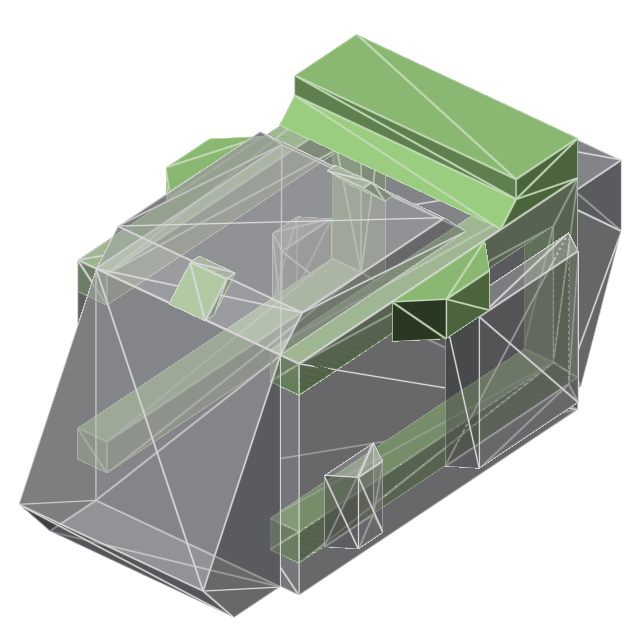
\includegraphics [
                height = 0.16\textheight,
                trim = {0cm 0 0cm 0},
                clip,
            ] {pics/ext_both_right.png}
            \captionof{figure} {Exhaust System.}
            \label{fig:}
        \end{figure}
    \end{minipage}
    \hfill
    \begin{minipage} {0.50\textwidth}
        The exhaust system of the Incubator plays major role in controlling the
        internal environment. It helps to regulate the \emph{temperature}, \emph{humidity}
        and \emph{air quality}. Temperature and humidity plays a major role in
        the proper germination of the seed. Since the incubator is an isolated system, it is
        important to replenish the air as \emph{$\mbox{CO}_2$} levels could become abnormal.
    \end{minipage}
\end{center}

% The entire exhaust system consists of three parts.
% One is a \emph{core block} that can act as a cooler, heater and as an exhaust based on the
% configuration. Then two dedicated coolers and two branches of exhaust pipes from both the
% side sides of the core block.

\subsection{Humidifiers and Humidifier Reservoir}

\begin{center}
    \begin{minipage} {0.49\textwidth}
        \begin{figure}[H]
            \centering
            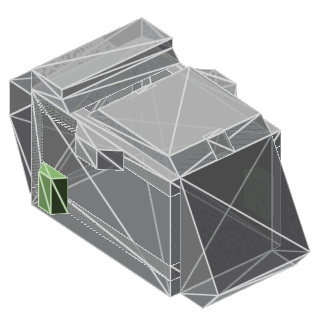
\includegraphics [
                height = 0.16\textheight,
                trim = {0cm 0 0cm 0},
                clip,
            ] {pics/hume_res_left.png}
            \captionof{figure} {Humidifier Reservoirs.}
            \label{fig:}
        \end{figure}
    \end{minipage}
    \hfill
    \begin{minipage} {0.50\textwidth}
        The incubator will have two internal \emph{piezoelectric humidifiers}. Water for these
        humidifiers will be stored in the humidifier reservoirs, which are placed
        outside the incubator for easy access by the user without the need to open the
        incubator.
    \end{minipage}
\end{center}

\subsection{Top and Side Hatches}

\begin{center}
    \begin{minipage} {0.49\textwidth}
        \begin{figure}[H]
            \centering
            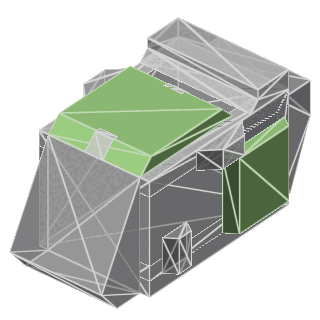
\includegraphics [
                height = 0.16\textheight,
                trim = {0cm 0 0cm 0},
                clip,
            ] {pics/hatch_both_right.png}
            \captionof{figure} {Top Hatch.}
            \label{fig:}
        \end{figure}
    \end{minipage}
    \hfill
    \begin{minipage} {0.50\textwidth}
        It is important to gradually expose the saplings to the outside environment to
        reduce stress. The top hatch helps achieve this. Once the saplings are ready to
        be planted outside, the incubator will slowly adjust its internal conditions to
        match the external environment and gradually open the top hatch.
    \end{minipage}
\end{center}

\subsection{Incubator Area}

\begin{center}
    \begin{minipage} {0.49\textwidth}
        \begin{figure}[H]
            \centering
            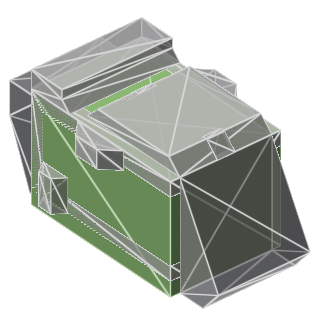
\includegraphics [
                height = 0.16\textheight,
                trim = {0cm 0 0cm 0},
                clip,
            ] {pics/inc_area_left.png}
            \captionof{figure} {Incubator Area.}
            \label{fig:}
        \end{figure}
    \end{minipage}
    \hfill
    \begin{minipage} {0.50\textwidth}
        The seeds are planted in this incubator area, which will be isolated from the
        outside world. It will provide optimal conditions for faster germination and
        for the seeds after germination. The incubator area will have dimensions of
        approximately 80 cm x 50 cm x 50 cm, allowing for the planting of around six
        seeds at a time.
    \end{minipage}
\end{center}

\subsection{Electronics Bay}

\begin{center}
    \begin{minipage} {0.49\textwidth}
        \begin{figure}[H]
            \centering
            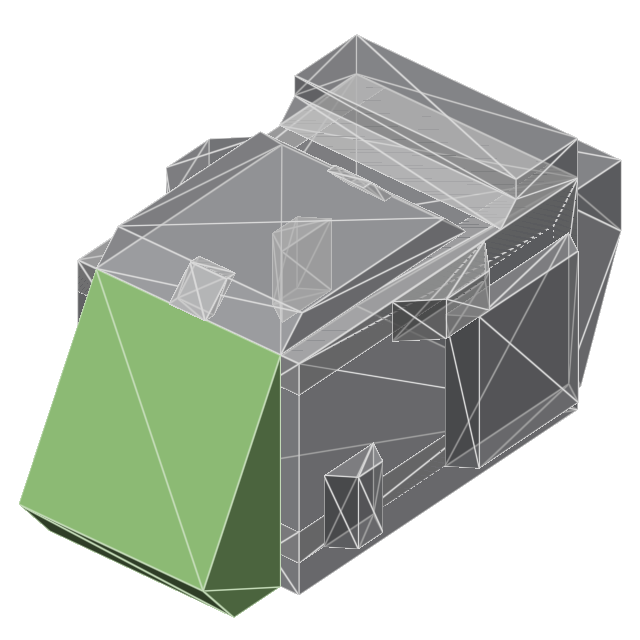
\includegraphics [
                height = 0.16\textheight,
                trim = {0cm 0 0cm 0},
                clip,
            ] {pics/elec_bay_right.png}
            \captionof{figure} {Electronics Bay.}
            \label{fig:}
        \end{figure}
    \end{minipage}
    \hfill
    \begin{minipage} {0.50\textwidth}
        It is important to isolate the electronic circuits of the incubator from the
        rest of the system. The electronics bay serves this purpose. Most of the
        electronic components, including the power supply, will be housed here,
        protecting them from water exposure and temperature variations.
    \end{minipage}
\end{center}

\subsection{Water and Fertilizer Reservoir}

\begin{center}
    \begin{minipage} {0.49\textwidth}
        \begin{figure}[H]
            \centering
            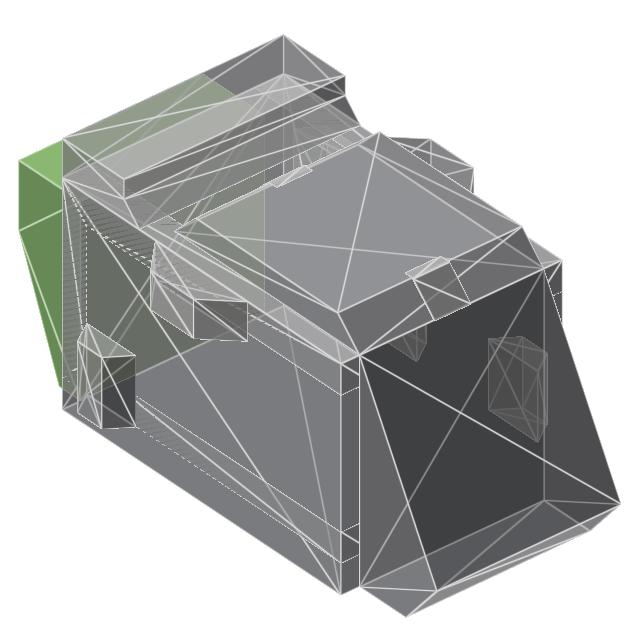
\includegraphics [
                height = 0.16\textheight,
                trim = {0cm 0 0cm 0},
                clip,
            ] {pics/water_res_left.png}
            \captionof{figure} {Water and Fertilizer Reservoir.}
            \label{fig:}
        \end{figure}
    \end{minipage}
    \hfill
    \begin{minipage} {0.50\textwidth}
        Water and fertilizer for the saplings are stored at the back of the incubator.
        The incubator can store up to 25 liters of water and 10 liters of fertilizer
        dissolved in water. These reservoirs are placed outside the incubator so that
        they can be refilled from the outside.
    \end{minipage}
\end{center}


% \subsection{Side Hatch}
%
% \begin{figure} [H]
%     \centering
%     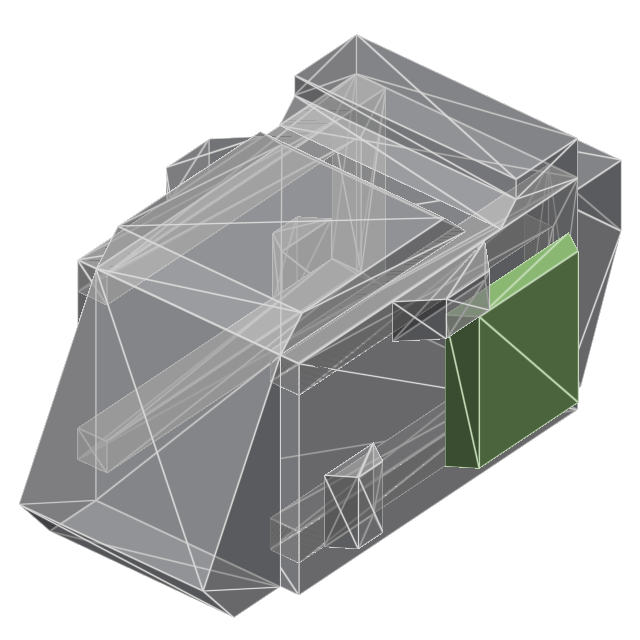
\includegraphics [
%         height = 0.3\textheight,
%     ] {pics/side_hatch_right.png}
%     \captionof{figure} {Side Hatch of the Incubator.}
%     \label{fig:}
% \end{figure}
%
% The side hatch provides another way to access the internals of the incubator more effectively.

\end{document}
